\documentclass[a4paper]{article}
\usepackage{amsfonts}
\usepackage{amsmath}
\usepackage{amssymb}
\usepackage{graphicx}
\usepackage{extarrows}

\newcommand{\integral}{\displaystyle\int}
\newcommand{\limit}{\lim\limits}

\begin{document}

\noindent \large Auteur: Seda Jusjajeva\\
\noindent \large Studierichting: Informatica\\
\noindent \large Oefeningenreeks 5E nr. 1\\

\medskip

\normalsize



$\left\{\begin{array}{l}
    x(t) = t^2 \\
    y(t) = 4t - t^3 \\
\end{array}\right.$ \\

$S = \integral^{t_2}_{t_1}|4t - t^3|(t^2)'dt$ \\

$= \integral^{t_2}_{t_1}|4t - t^3|2tdt$ \\

$\integral|4t - t^3|2tdt$ \\

$= \integral(8t^2 - 2t^4)dt $\\

$= 8\integral t^2dt - 2\integral t^4dt$\\

$= \dfrac{8t^3}{3} - \dfrac{2t^5}{5} + c$\\

$|4t - t^3| = 0 \vee t^2 = 0$ \\

$\Leftrightarrow |t(4 - t^2)| = 0 \vee t = 0$ \\

$\Leftrightarrow t = -2 \vee t = 0 \vee t = 2$ \\

\begin{figure}[h]
	\centering
	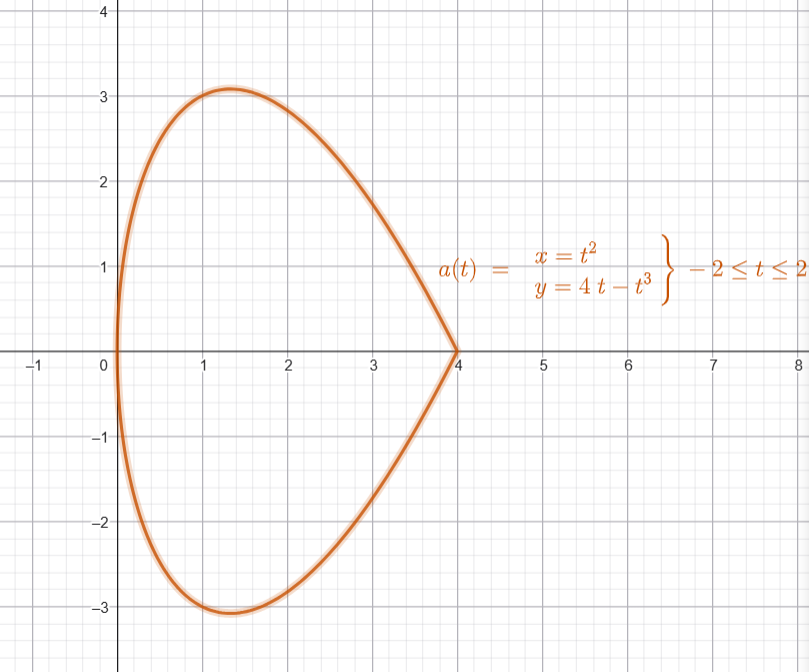
\includegraphics[width=8cm]{5E-1-seda.jusjajeva.INF.png}
\end{figure}

$2\integral_0^2 |4t - t^3|2tdt$ \\

$= 2\left[\dfrac{8t^3}{3} - \dfrac{2t^5}{5}\right]_{0}^{2} = 2\cdot\left(\dfrac{8\cdot2^3}{3} - \dfrac{2\cdot2^5}{5}\right) - 2\cdot0 = \dfrac{640}{15} - \dfrac{384}{15} = \dfrac{256}{15}$ \\



\begin{thebibliography}{999}
%\bibitem{a} Referentie
\end{thebibliography}
\end{document}